\scanpage{75}

% top, lines 1–8
de trièdres $H$. Notons que la cat. des hexagones combinatoires équivaut à $(\mathrm{Ens})_3\times(\mathrm{Ens})_2$, à un hexagone correspondant l'\deleted{\unsure{él.}}\inserted{ens} $\deleted{\unsure{\xi|t}}\tau$ de ses trois diagonales, et l'ens $\varepsilon$ des deux triangles inscrits (triangles d'éléments biliés) -- et au couple $\tau,\varepsilon$ correspondant l'hexagone \deleted{\unsure{h}} dont l'ens des sommets est $\tau\times\varepsilon$, \deleted{\unsure{$h$}} et les sommets $(a,\alpha)$ et $(b,\beta)$ sont liés ssi $a\ne b$ $\alpha\ne\beta$.

% upper-middle, lines 8–13
Ceci posé, l'ens $\unsure{\mathrm{Aut}|\mathrm{Or}}(h)$ d'un hexagone $h$ s'identifie à l'ens des orientations du $\tau$ associé (si cette orientation est définie par $u\in\unsure{\mathrm{Aut}}\tau$, alors celle de $h\simeq\tau\times\varepsilon$ est donné par $u\times u_\varepsilon$, où $u_\varepsilon$ est l'autom. non identique de $\varepsilon$).

% middle, lines 14–16
Or explicitons \inserted{(dans le cas d'un trièdre $t$ donné.)} les relations entre les deux hexagones $h$ et $H$ qu'elle définit en termes d'un ens du type $(333)$

% lower left, adjacent to text
\diagram{\begin{tikzcd}[ampersand replacement=\&,column sep=0pt]
I\arrow[d,"p"']\&{}=\displaystyle\coprod_{\alpha\in\Lambda}I_\alpha.\\
\Lambda\&
\end{tikzcd}}

% lower right, lines 17–20
Un trièdre correspond à la donnée d'un couple $i,\beta$, $i\in I$, $\beta\in\Lambda$, $\beta\ne p(i)=\alpha$, cf figure donc si $\gamma\inI$ est $\ne\alpha,\beta$, alors l'ens.

% lower left, below Λ
\figure{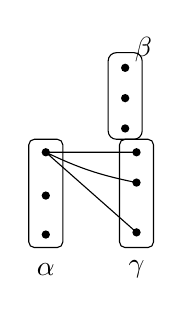
\begin{tikzpicture}[x=0.72cm,y=0.55cm]
\draw[rounded corners=3pt] (1.1,2.5) rectangle (1.7,4.5);
\draw[rounded corners=2pt] (-.3,0) rectangle (.3,2.5);
\draw[rounded corners=2pt] (1.3,0) rectangle (1.9,2.5);
\foreach \x/\y in {1.4/4.15,1.4/3.45,1.4/2.75,0/2.2,0/1.2,0/.3,1.6/2.2,1.6/1.5,1.6/.35}{\fill (\x,\y) circle (1.5pt);}
\draw (0,2.2)--(1.6,2.2) (0,2.2) to[bend right=7] (1.6,1.5) (0,2.2)--(1.6,.35);
\node at (1.72,4.58) {$\beta$};\node at (0,-.5) {$\alpha$};\node at (1.6,-.5) {$\gamma$};
\end{tikzpicture}}

% lower and foot, lines 21–25
à trois éléments associé à $h$, qui n'est autre que $t$ lui-$=$, s'identifie à $I_\gamma$. Les deux trièdres \inserted{$t',t''$} parallèles à $t$ et $\ne t$ sont évidemment celles données par $(j,\beta)$, $j\in I_\alpha\setminus\{i\}$, donc $\varepsilon\simeq I_\alpha-\{i\}$, donc

% foot, last line
\[
h\Leftrightarrow(I_\gamma,I_\alpha\setminus\{i\})
\]

% archive sheet number: 74
